
\begin{frame}
   \frametitle{Path Distribution via the Partition Function}
   
   \begin{itemize}
   \item
   Sampling weight functions and solving the corresponding SP problems
   can be expensive.
   
   \pause
   \item
   How else can we efficiently generate a reasonable distribution
   over potential paths?
   \end{itemize}
   
   \pause
   \begin{equation*}
      P: \mbox{set of all paths from $v_s$ to $v_t$}
   \end{equation*}%
   \pause%
   \vspace{-0.3cm}
   \begin{equation*}
      \arraycolsep=1pt
      \begin{array}{ll}
      \mathcal{D}_p : & \mbox{path distribution with PDF } \\
      & f(p) \propto \exp( - \beta \, \mbox{len}(p, w_{\ms{lazy}}) ). \\
      \end{array}
   \end{equation*}
   
   \pause
   \vspace{0.3cm}
   \begin{itemize}
   \item At each iteration,
   the shortest path in $P$
   (which is chosen as the LazySP candidate path)
   is most likely under $\mathcal{D}_p$ ...
   
   \pause
   \item ... but other paths also have probability mass,
      with longer paths exponentially less likely.
   \end{itemize}
   
\end{frame}

\begin{frame}
   \frametitle{Path Distribution via the Partition Function}
   \begin{tikzpicture}
      \draw[step=1,black!15,very thin,opacity=\gridopacity] (0,0) grid (12,8);
      \tikzset{>=latex}
   
      \node at (6,7.5) {
         Examples of the edge probabilities for various values of $\beta$:
      };
      
      \only<2->{
      \node (empty50) at (3,5.5) {\includegraphics{build/lazysp-selscores/empty-50}};
      \node[anchor=north west, below right=0.2cm of empty50.north west,font=\small] {$\beta=50$};
      }
      \only<3->{
      \node (empty33) at (6,5.5) {\includegraphics{build/lazysp-selscores/empty-33}};
      \node[anchor=north west, below right=0.2cm of empty33.north west,font=\small] {$\beta=33$};
      }
      \only<4->{
      \node (empty28) at (9,5.5) {\includegraphics{build/lazysp-selscores/empty-28}};
      \node[anchor=north west, below right=0.2cm of empty28.north west,font=\small] {$\beta=28$};
      }
      
      \only<5->{
      \node (gap50) at (3,2.3) {\includegraphics{build/lazysp-selscores/gap-50}};
      \node[anchor=north west, below right=0.2cm of gap50.north west,font=\small] {$\beta=50$};
      }
      \only<6->{
      \node (gap33) at (6,2.3) {\includegraphics{build/lazysp-selscores/gap-33}};
      \node[anchor=north west, below right=0.2cm of gap33.north west,font=\small] {$\beta=33$};
      }
      \only<7->{
      \node (gap28) at (9,2.3) {\includegraphics{build/lazysp-selscores/gap-28}};
      \node[anchor=north west, below right=0.2cm of gap28.north west,font=\small] {$\beta=28$};
      }
   
   \end{tikzpicture}
\end{frame}

\begin{frame}
   \frametitle{Partition Function: Incremental Formulation}
   
   Efficient implementation of the partition function selector
   requires an incremental algorithm for calculating $Z_{st}$ over $G$.
   
   \begin{equation*}
      P_{xy}: \mbox{set of all paths from $v_x$ to $v_y$}
   \end{equation*}
   \begin{equation*}
      Z_{xy} = \sum_{p \in P_{xy}} \exp( - \beta \, \mbox{len}(p) )
   \end{equation*}
   
   \pause
   Consider two directed graphs, $G=(V,E)$ and $G'=(V,E')$,
   with $E' = E \cup \{ e'_{ab} \}$
   and $z'_{ab} = \exp(-\beta w(e'_{ab}))$.
   Suppose that the values $Z_{xy}$ are known for all pairs $x,y$.
   Then we can write:
   \pause
   \begin{equation*}
      \arraycolsep=1pt
      \def\arraystretch{1.8}
      \begin{array}{ll}
      Z'_{xy}
         & = \left[ Z_{xy} \right]
         + \left[ Z_{xa} \, z'_{ab} \, Z_{by} \right]
         + \left[ Z_{xa} \, z'_{ab} \, Z_{ba} \, z'_{ab} \, Z_{by} \right]
         + \dots \\
      \pause
      & = Z_{xy} + \frac{\displaystyle Z_{xa} Z_{by}}{\displaystyle 1 / z'_{ab} - Z_{ba}}
      \end{array}
   \end{equation*}
   
\end{frame}

\begin{frame}
   \frametitle{Distance Functions}
   \begin{tikzpicture}[font=\small]
      \tikzset{>=latex} % arrow heads
      \draw[step=1,black!15,very thin,opacity=\gridopacity] (0,0) grid (12,8);

      \begin{scope}[shift={(4.25,5.2)}]
         \node[inner sep=0pt,anchor=south west] {%
            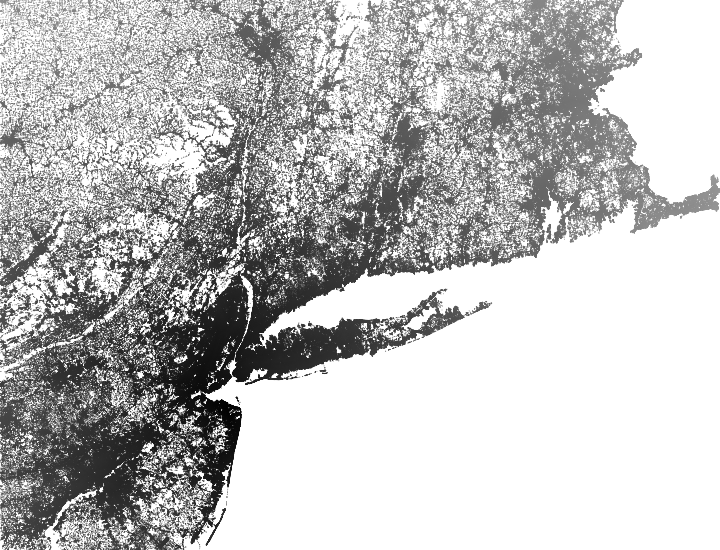
\includegraphics[width=3.5cm]{figs/incbi-road-ne/singleshot/example-dijkstraall.png}};
         \coordinate (s) at (1.226,0.63);
         %\coordinate (t) at (2.751,1.96);
         \node (slab) at (1.75,0.42) {$s$};
         %\node (tlab) at (2.8,1.05) {$t$};
         \draw[->,thick] (slab) -- (s);
         %\draw[->,thick] (tlab) -- (t);
      \end{scope}

      \node[fill=blue!10] at (3,4.0) {\begin{minipage}{5.5cm}
         Definition:
         \[
            d^*(v) = \min_{p \in P_{sv}} \mbox{len}(p,w)
         \]
      \end{minipage}};
      \node[fill=blue!10] at (9,4.0) {\begin{minipage}{5.5cm}
         Local characterization:
         \[
            \arraycolsep=1.4pt
            d^*(v) = 
            \left\{ \begin{array}{cl}
               0 & v = s \\
               \displaystyle\min_{e_{uv}} d^*(u)\!+\!w(e_{uv}) & v \neq s \\
            \end{array} \right.
         \]
      \end{minipage}};

      

      %\only<2->{
      %\node at (6,3.3) {Key: Understanding properties of an approximation $d$.};
      %}

      \only<2->{
      \node[fill=blue!10,minimum width=2cm,align=center] (d) at (6,1.75)
         {Approximation\\$d : V \rightarrow \mathbb{R}$};
      }

      \only<3->{
         \node[align=center] at (6,0.75) {Properties of $d$?};
      }

      \only<4->{
      \node[draw=black!50,densely dashed,minimum width=2cm,align=center] (dprime) at (9,1.75)
         {Approximation\\$d\:\!' : V \rightarrow \mathbb{R}$};
      \draw[->,very thick] (d) -- (dprime);
      }

   \end{tikzpicture}
\end{frame}

\begin{frame}
   \frametitle{Approximating the Distance Function: Non-Incremental}
   \begin{tikzpicture}[font=\small]
      \tikzset{>=latex} % arrow heads
      \draw[step=1,black!15,very thin,opacity=\gridopacity] (0,0) grid (12,8);

      \node[fill=blue!10] at (3,7.0) {\begin{minipage}{5.5cm}
         Definition:
         \[
            d^*(v) = \min_{p \in P_{sv}} \mbox{len}(p,w)
         \]
      \end{minipage}};
      \node[fill=blue!10] at (9,7.0) {\begin{minipage}{5.5cm}
         Local characterization:
         \[
            \arraycolsep=1.4pt
            d^*(v) = 
            \left\{ \begin{array}{cl}
               0 & v = s \\
               \displaystyle\min_{e_{uv}} d^*(u)\!+\!w(e_{uv}) & v \neq s \\
            \end{array} \right.
         \]
      \end{minipage}};

      \only<2->{
      \node[fill=black!5,minimum width=5.75cm] at (3,5.5) {\strut Non-Incremental Search};
      \node[fill=blue!10,align=center] at (1,4.6) {Fixed\\$w \geq 0$};
      }
      \only<3->{
      \node[fill=blue!10,align=center] at (3.5,4.6) {Approximation\\$d : V \rightarrow \mathbb{R}$};
      }
      \only<4->{
      \node[fill=blue!10,minimum width=5.75cm,minimum height=2.5cm,anchor=north] (tens) at (3,4.0) {};
      \only<7->{
      \node[fill=red!20,minimum width=5.75cm,minimum height=0.5cm] at (3,1.75) {};
      }
      \node[anchor=north] at (tens.north) {\begin{minipage}{5.5cm}
         Constraints on $d$:
         \vspace{-0.2cm}
         \[
             d^*(v) \leq d(v)
         \]
         \vspace{-0.6cm}
         \[
             d(s) = 0
         \]
         \vspace{-0.5cm}
         \[
            \min_{e_{uv}} d(u) + w(e_{uv}) \leq d(v) \quad v \neq s
         \]
         \vspace{-0.3cm}
         \[
            d(u) + w(e_{uv}) \geq d(v)
         \]
         %Ordering, Early Term if $w \geq 0$
      \end{minipage}};
      }

      \only<5>{
         \node[fill=blue!10] (equal) at (9,2.7) {$d = d^*$};
         \draw[->,very thick] (tens) -- (equal);
      }

      % trust region
      \only<6->{
         \node at (9,3.7) {\includegraphics[width=4.5cm]{build/ibid-dijkstra-trust-build,init}};
      }
      \only<8->{
         \node at (9,3.7) {\includegraphics[width=4.5cm]{build/ibid-dijkstra-trust-build,wtensioned}};
      }
      \only<9->{
         \node at (9,3.7) {\includegraphics[width=4.5cm]{build/ibid-dijkstra-trust-build,wtrust}};
      }

      \only<10->{
      \node[fill=blue!10,align=center] at (3,0.7) {
         TR: If $w \geq 0$ and $D$ is the minimal\\
         $d(u)$ among tensioned edges $e_{uv}$,\\
         then any $v$ with $d(v) \leq D$ is correct.
      };
      }

      \only<11->{
         \node[fill=green!10,align=center] at (7.7,0.75) {Relaxation\\Ordering!};
      }
      \only<12->{
         \node[fill=green!10,align=center] at (10.3,0.75) {Early\\Termination!};
      }

   \end{tikzpicture}
\end{frame}

\begin{frame}
   \frametitle{Approximating the Distance Function: Incremental}
   \begin{tikzpicture}[font=\small]
      \tikzset{>=latex} % arrow heads
      \draw[step=1,black!15,very thin,opacity=\gridopacity] (0,0) grid (12,8);

      \node[fill=blue!10] at (3,7.0) {\begin{minipage}{5.5cm}
         Definition:
         \[
            d^*(v) = \min_{p \in P_{sv}} \mbox{len}(p,w)
         \]
      \end{minipage}};
      \node[fill=blue!10] at (9,7.0) {\begin{minipage}{5.5cm}
         Local characterization:
         \[
            \arraycolsep=1.4pt
            d^*(v) = 
            \left\{ \begin{array}{cl}
               0 & v = s \\
               \displaystyle\min_{e_{uv}} d^*(u)\!+\!w(e_{uv}) & v \neq s \\
            \end{array} \right.
         \]
      \end{minipage}};

      \only<-5>{
      \node[fill=black!5,minimum width=5.75cm] at (3,5.5) {\strut Non-Incremental Search};
      \node[fill=blue!10,align=center] at (1,4.6) {Fixed\\$w \geq 0$};
      \node[fill=blue!10,align=center] at (3.5,4.6) {Approximation\\$d : V \rightarrow \mathbb{R}$};
      \node[fill=blue!10,minimum width=5.75cm,minimum height=2.5cm,anchor=north] (tens) at (3,4.0) {};
      \node[fill=red!20,minimum width=5.75cm,minimum height=0.5cm] at (3,1.75) {};
      \node[anchor=north] at (tens.north) {\begin{minipage}{5.5cm}
         Constraints on $d$:
         \vspace{-0.2cm}
         \[
             d^*(v) \leq d(v)
         \]
         \vspace{-0.6cm}
         \[
             d(s) = 0
         \]
         \vspace{-0.5cm}
         \[
            \min_{e_{uv}} d(u) + w(e_{uv}) \leq d(v) \quad v \neq s
         \]
         \vspace{-0.3cm}
         \[
            d(u) + w(e_{uv}) \geq d(v)
         \]
         %Ordering, Early Term if $w \geq 0$
      \end{minipage}};
      \fill[white,opacity=0.5] (0,1) rectangle (6,6);
      }

      \node[fill=black!5,minimum width=5.75cm] at (9,5.5) {\strut Incremental Search};

      \only<2->{
      \node[fill=blue!10,align=center] at (7,4.6) {Dynamic\\$w > 0$};
      \node[fill=blue!10,align=center] at (9.5,4.6) {Approximation\\$d : V \rightarrow \mathbb{R}$};
      }

      \only<3-4>{
      \node[fill=blue!10,minimum width=5.75cm,minimum height=2.5cm,anchor=north] (incons) at (9,4.0) {};
      \node[fill=red!20,minimum width=5.75cm,minimum height=0.5cm] at (9,1.75) {};
      \node[anchor=north] at (incons.north) {\begin{minipage}{5.5cm}
         Constraints on $d$:
         \vspace{-0.2cm}
         \[
             d^*(v) \leq d(v)
         \]
         \vspace{-0.6cm}
         \[
             d(s) = 0
         \]
         \vspace{-0.5cm}
         \[
            \min_{e_{uv}} d(u) + w(e_{uv}) \leq d(v) \quad v \neq s
         \]
         \vspace{-0.3cm}
         \[
            d(u) + w(e_{uv}) \geq d(v)
         \]
         %Ordering, Early Term if $w \geq 0$
      \end{minipage}};
      }
      \only<4>{
         \draw[red,ultra thick] (9,3.25) ellipse (1cm and 0.5cm);
         \draw[red,ultra thick] (8.2,3.55) -- (9.8,2.95);
         \draw[red,ultra thick] (8.2,2.95) -- (9.8,3.55);
      }

      \only<5->{
      \node[fill=blue!10,minimum width=5.75cm,minimum height=2.0cm,anchor=north] (incons) at (9,4.0) {};
      \only<7->{
      \node[fill=red!20,minimum width=5.75cm,minimum height=0.5cm] at (9,2.25) {};
      }
      \node[anchor=north] at (incons.north) {\begin{minipage}{5.5cm}
         Constraints on $d$:
         \vspace{-0.2cm}
         \[
            \arraycolsep=1.4pt
            r(v) = 
            \left\{ \begin{array}{cl}
               0 & v = s \\
               \displaystyle\min_{e_{uv}} d(u)\!+\!w(e_{uv}) & v \neq s \\
            \end{array} \right.
         \]
         \vspace{-0.3cm}
         \[
             d(v) = r(v)
         \]
         %Ordering, Early Term if $w \geq 0$
      \end{minipage}};
      }

      \only<6-7>{
         \node at (3,3.7) {\includegraphics[width=4.5cm]{build/ibid-dijkstra-trust-build,init}};
      }
      \only<8>{
         \node at (3,3.7) {\includegraphics[width=4.5cm]{build/ibid-dijkstra-trust-build,wincons}};
      }
      \only<9->{
         \node at (3,3.7) {\includegraphics[width=4.5cm]{build/ibid-dijkstra-trust-build,winctrust}};
      }
      
      \only<10->{
      \node[fill=blue!10,align=center] at (9,1.0) {
         TR: If $w > 0$ and $K$ is the minimal \\
         $k(v) = \min(d(v), r(v))$ among $V_{\ms{incons}}$, \\
         then any consistent $v$ \\
         with $d(v) \leq K$ is correct.
      };
      }

      \only<11->{
         \node[fill=green!10,align=center] at (1.7,0.75) {Relaxation\\Ordering!};
         \node[fill=green!10,align=center] at (4.3,0.75) {Early\\Termination!};
      }

   \end{tikzpicture}
\end{frame}

\begin{frame}
   \frametitle{Trust Regions}
   \begin{tikzpicture}[font=\small]
      \tikzset{>=latex} % arrow heads
      \draw[step=1,black!15,very thin,opacity=\gridopacity] (0,0) grid (12,8);

      % complete side
      \node[fill=black!5,minimum width=5.75cm] at (3,7.5) {\strut Non-Incremental Search};
      \node[fill=blue!10,align=center] at (1,6.6) {Fixed\\$w \geq 0$};
      \node[fill=blue!10,align=center] at (3.5,6.6) {Approximation\\$d : V \rightarrow \mathbb{R}$};
      \node[fill=blue!10,minimum width=5.75cm,minimum height=2.5cm,anchor=north] (tens) at (3,6.0) {};
      \node[fill=red!20,minimum width=5.75cm,minimum height=0.5cm] at (3,3.75) {};
      \node[anchor=north] at (tens.north) {\begin{minipage}{5.5cm}
         Constraints on $d$:
         \vspace{-0.2cm}
         \[
             d^*(v) \leq d(v)
         \]
         \vspace{-0.6cm}
         \[
             d(s) = 0
         \]
         \vspace{-0.5cm}
         \[
            \min_{e_{uv}} d(u) + w(e_{uv}) \leq d(v) \quad v \neq s
         \]
         \vspace{-0.3cm}
         \[
            d(u) + w(e_{uv}) \geq d(v)
         \]
         %Ordering, Early Term if $w \geq 0$
      \end{minipage}};
      \node[fill=blue!10,align=center] at (3,2.75) {
         TR: If $w \geq 0$ and $D$ is the minimal\\
         $d(u)$ among tensioned edges $e_{uv}$,\\
         then any $v$ with $d(v) \leq D$ is correct.
      };
      \node at (3,1.05) {\includegraphics[width=2.5cm]{build/ibid-dijkstra-trust-build,wtrust}};

      % incremental side
      \node[fill=black!5,minimum width=5.75cm] at (9,7.5) {\strut Incremental Search};
      \node[fill=blue!10,align=center] at (7,6.6) {Dynamic\\$w > 0$};
      \node[fill=blue!10,align=center] at (9.5,6.6) {Approximation\\$d : V \rightarrow \mathbb{R}$};
      \node[fill=blue!10,minimum width=5.75cm,minimum height=2.0cm,anchor=north] (incons) at (9,6.0) {};
      \node[fill=red!20,minimum width=5.75cm,minimum height=0.5cm] at (9,4.25) {};
      \node[anchor=north] at (incons.north) {\begin{minipage}{5.5cm}
         Constraints on $d$:
         \vspace{-0.2cm}
         \[
            \arraycolsep=1.4pt
            r(v) = 
            \left\{ \begin{array}{cl}
               0 & v = s \\
               \displaystyle\min_{e_{uv}} d(u)\!+\!w(e_{uv}) & v \neq s \\
            \end{array} \right.
         \]
         \vspace{-0.3cm}
         \[
             d(v) = r(v)
         \]
         %Ordering, Early Term if $w \geq 0$
      \end{minipage}};
      \node[fill=blue!10,align=center] at (9,3.0) {
         TR: If $w > 0$ and $K$ is the minimal \\
         $k(v) = \min(d(v), r(v))$ among $V_{\ms{incons}}$, \\
         then any consistent $v$ \\
         with $d(v) \leq K$ is correct.
      };
      \node at (9,1.05) {\includegraphics[width=2.5cm]{build/ibid-dijkstra-trust-build,winctrust}};

   \end{tikzpicture}
\end{frame}

%\begin{frame}
%   \frametitle{Trust Regions}
%   \begin{tikzpicture}[font=\small]
%      \tikzset{>=latex} % arrow heads
%      \draw[step=1,black!15,very thin,opacity=\gridopacity] (0,0) grid (12,8);
%
%      % ordering problems
%      %\begin{scope}[shift={(1.5,5.5)}]
%      %\begin{scope}[shift={(0,0)}]
%      %   \node[fill=black,circle,inner sep=1.2pt] (a) at (0,0) {};
%      %   \node[fill=black,circle,inner sep=1.2pt] (b) at (1.5,0) {};
%      %   \node[fill=black,circle,inner sep=1.2pt] (c) at (3.0,0) {};
%      %   \draw[->,densely dashed] (a) -- (b) node[midway,fill=white,circle,inner sep=1pt] {1};
%      %   \draw[->,densely dashed] (b) -- (c) node[midway,fill=white,circle,inner sep=1pt] {1};
%      %   
%      %   \node[above=-0.00cm of a] {$a$};
%      %   \node[above=-0.00cm of b] {$b$};
%      %   \node[above=-0.00cm of c] {$c$};
%      %
%      %   \node[below=0.05cm of a] {$d=0$};
%      %   \node[below=0.05cm of b] {$d=2$};
%      %   \node[below=0.05cm of c] {$d=4$};
%      %\end{scope}
%      %
%      %\begin{scope}[shift={(0,-1)}]
%      %   \node[fill=black,circle,inner sep=1.2pt] (a) at (0,0) {};
%      %   \node[fill=black,circle,inner sep=1.2pt] (b) at (1.5,0) {};
%      %   \node[fill=black,circle,inner sep=1.2pt] (c) at (3.0,0) {};
%      %   \draw[->,densely dashed] (a) -- (b) node[midway,fill=white,circle,inner sep=1pt] {1};
%      %   \draw[line width=0.10cm,black!10] (b) -- (c) node[midway,fill=white,circle,inner sep=1pt] {1};
%      %   \draw[->] (b) -- (c) node[midway,fill=white,circle,inner sep=1pt] {1};
%      %
%      %   \node[below=0.05cm of a] {$d=0$};
%      %   \node[below=0.05cm of b] {$d=2$};
%      %   \node[below=0.05cm of c] {$d=3$};
%      %\end{scope}
%      %
%      %\begin{scope}[shift={(0,-2)}]
%      %   \node[fill=black,circle,inner sep=1.2pt] (a) at (0,0) {};
%      %   \node[fill=black,circle,inner sep=1.2pt] (b) at (1.5,0) {};
%      %   \node[fill=black,circle,inner sep=1.2pt] (c) at (3.0,0) {};
%      %   \draw[line width=0.10cm,black!10] (a) -- (b) node[midway,fill=white,circle,inner sep=1pt] {1};
%      %   \draw[->] (a) -- (b) node[midway,fill=white,circle,inner sep=1pt] {1};
%      %   \draw[->,densely dashed] (b) -- (c) node[midway,fill=white,circle,inner sep=1pt] {1};
%      %   
%      %   \node[below=0.05cm of a] {$d=0$};
%      %   \node[below=0.05cm of b] {$d=1$};
%      %   \node[below=0.05cm of c] {$d=3$};
%      %\end{scope}
%      %
%      %\begin{scope}[shift={(0,-3)}]
%      %   \node[fill=black,circle,inner sep=1.2pt] (a) at (0,0) {};
%      %   \node[fill=black,circle,inner sep=1.2pt] (b) at (1.5,0) {};
%      %   \node[fill=black,circle,inner sep=1.2pt] (c) at (3.0,0) {};
%      %   \draw[->] (a) -- (b) node[midway,fill=white,circle,inner sep=1pt] {1};
%      %   \draw[line width=0.10cm,black!10] (b) -- (c) node[midway,fill=white,circle,inner sep=1pt] {1};
%      %   \draw[->] (b) -- (c) node[midway,fill=white,circle,inner sep=1pt] {1};
%      %   
%      %   \node[below=0.05cm of a] {$d=0$};
%      %   \node[below=0.05cm of b] {$d=1$};
%      %   \node[below=0.05cm of c] {$d=2$};
%      %\end{scope}
%      %\end{scope}
%
%      \node[fill=blue!10] at (3,7.25) {$d : V \rightarrow \mathbb{R}$};
%
%      \node[fill=blue!10,minimum width=5.75cm,minimum height=3.5cm] (erelax) at (3,5) {};
%      \node[anchor=north] at (erelax.north) {\begin{minipage}{5.5cm}
%         Tensioned Approximation $d$:
%         \vspace{-0.2cm}
%         \[
%             d^*(v) \leq d(v)
%         \]
%         \vspace{-0.6cm}
%         \[
%             d(s) = 0
%         \]
%         \vspace{-0.5cm}
%         \[
%            \min_{e_{uv}} d(u) + w(e_{uv}) \leq d(v)
%         \]
%         \vspace{-0.4cm}
%         \[
%            d(u) + w(e_{uv}) \geq d(v) [RELAXED]
%         \]
%         \only<2->{Ordering, Early Term if $w \geq 0$}
%      \end{minipage}};
%
%      % trust region
%      \node at (9,6.0) {\includegraphics[width=4.5cm]{build/ibid-dijkstra-trust}};
%
%
%      \only<3->{
%      \node[fill=blue!10,align=center] at (5,2.5) {
%         Trust Region:\\
%         If $w \geq 0$ and $D$ is the minimum $d(u)$ among tensioned edges $e_{uv}$,\\
%         then any $v$ with $d(v) \leq D$ is correct.
%      };
%      }
%
%      \only<4->{
%         \node[fill=blue!10,align=center] at (5,1.0) {
%            Algorithm: Order edges by $d(u)$ (Dijkstra's algorithm).
%         };
%
%         \node at (10.9,2.9) {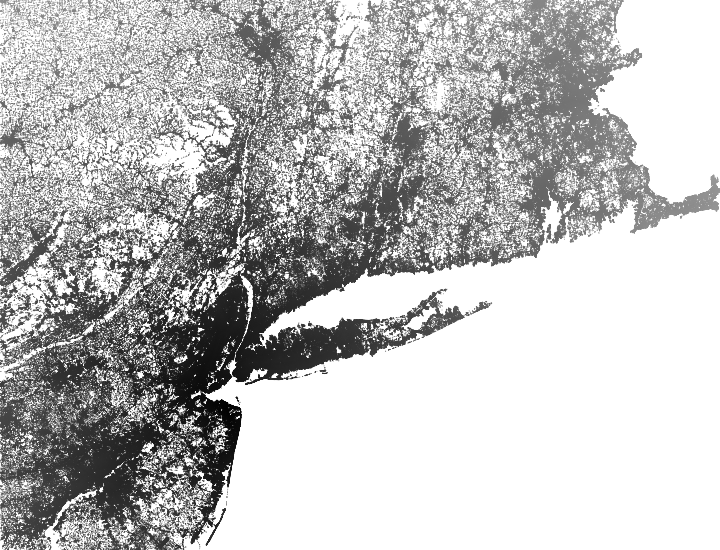
\includegraphics[width=2cm]{figs/incbi-road-ne/singleshot/example-dijkstraall.png}};
%         \node at (10.9,1.1) {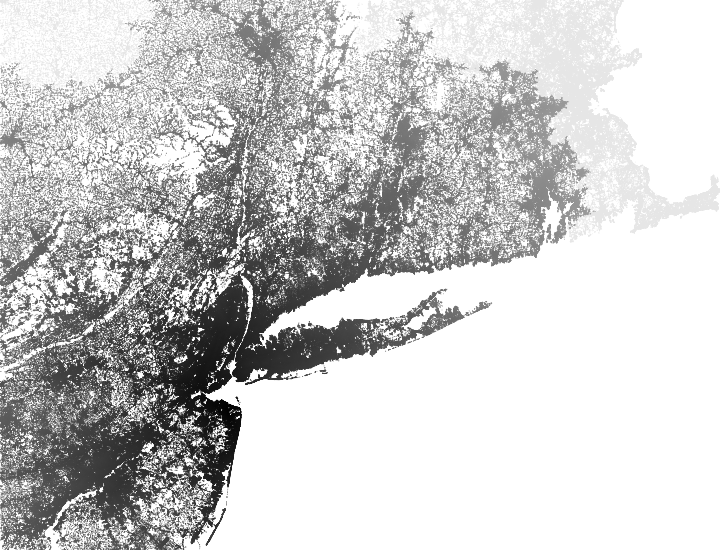
\includegraphics[width=2cm]{figs/incbi-road-ne/singleshot/example-dijkstra.png}};
%
%
%         \node[fill=blue!10,minimum width=5.75cm,minimum height=1.0cm] (erelax) at (3,0.7) {};
%         \node[anchor=north] at (erelax.north) {\begin{minipage}{5.5cm}
%            Terminate when $d(t) \leq D$.
%
%            $p$: Walk backwards on $d$ from $t$.
%         \end{minipage}};
%      }
%      
%   \end{tikzpicture}
%\end{frame}

\begin{frame}
   \frametitle{Incremental Bidirectional Dijkatra's Algorithm (IBiD)}
   \begin{tikzpicture}[font=\small]
      \tikzset{>=latex} % arrow heads
      \draw[step=1,black!15,very thin,opacity=\gridopacity] (0,0) grid (12,8);

      \node at (6,5.9) {\includegraphics{build/ibid-bidijkstra-sep}};

      \only<2->{
      \node[fill=blue!5,align=center,minimum width=3.5cm] at (1.8,3.3) {$Q_s$: $d_s$ Inconsistent\\Vertex Queue};
      }
      \only<3->{
      \node[inner sep=0pt,align=center] at (1.8,2.2) {$u$ on $Q_s$ iff:\\$d_s(u)\!\neq\!r_s(u)$};
      }
      \only<4->{
      \node[inner sep=0pt,align=center] at (1.8,1.1) {$Q_s$ sorted by:\\$k_s(u)\!=\!\min(d_s(u),\!r_s(u))$};
      }

      \only<5->{
      \node[fill=red!5,align=center,minimum width=3.5cm] at (10.2,3.3) {$Q_t$: $d_t$ Inconsistent\\Vertex Queue};
      \node[inner sep=0pt,align=center] at (10.2,2.2) {$v$ on $Q_t$ iff:\\$d_t(v)\!\neq\!r_t(v)$};
      \node[inner sep=0pt,align=center] at (10.2,1.1) {$Q_t$ sorted by;\\$k_t(v)\!=\!\min(d_t(v),\!r_t(v))$};
      }

      \only<6->{
      \node[fill=green!10,align=center,minimum width=4.2cm] at (6,3.3) {$Q_c$: Connection\\Edge Queue};
      }
      \only<7->{
      \node[inner sep=0pt,align=center] at (6,2.2) {
         $e_{uv}$ on $Q_c$ iff:\\
         $d_s(u) = r_s(u); \; d_t(v) = r_t(v)$\\
         $d_s(u) \leq K_s; \; d_t(v) \leq K_t$};
      }
      \only<8->{
      \node[inner sep=0pt,align=center] at (6,1.1) {
         $Q_c$ sorted by:\\
         $d_s(u) + w(e_{uv}) + d_t(v)$};
      }
      \only<9->{
      \node[fill=green!15] at (6,0.3) {
         Terminate when $Q_c.\mbox{\sc TopKey} \leq K_s + K_t$.};
      }

   \end{tikzpicture}
\end{frame}

\begin{frame}
   \frametitle{LazySP Partition Function Examples}
   \begin{tikzpicture}[font=\small]
      \draw[step=1,black!15,very thin,opacity=\gridopacity] (0,0) grid (12,8);
      \tikzset{>=latex}
   
      \node at (6,7.5) {
         Examples of the edge probabilities for various values of $\beta$:
      };

      \only<2->{
      \node (gap50) at (3,5.5) {\includegraphics{build/lazysp-selscores/gap-50}};
      \node[anchor=north west, below right=0.2cm of gap50.north west,font=\small] {$\beta=50$};
      }
      \only<3->{
      \node (gap33) at (6,5.5) {\includegraphics{build/lazysp-selscores/gap-33}};
      \node[anchor=north west, below right=0.2cm of gap33.north west,font=\small] {$\beta=33$};
      }
      \only<4->{
      \node (gap28) at (9,5.5) {\includegraphics{build/lazysp-selscores/gap-28}};
      \node[anchor=north west, below right=0.2cm of gap28.north west,font=\small] {$\beta=28$};
      }
      
      \only<5->{
      \node (empty50) at (3,2.3) {\includegraphics{build/lazysp-selscores/empty-50}};
      \node[anchor=north west, below right=0.2cm of empty50.north west,font=\small] {$\beta=50$};
      }
      \only<6->{
      \node (empty33) at (6,2.3) {\includegraphics{build/lazysp-selscores/empty-33}};
      \node[anchor=north west, below right=0.2cm of empty33.north west,font=\small] {$\beta=33$};
      }
      \only<7->{
      \node (empty28) at (9,2.3) {\includegraphics{build/lazysp-selscores/empty-28}};
      \node[anchor=north west, below right=0.2cm of empty28.north west,font=\small] {$\beta=28$};
      }
   
   \end{tikzpicture}
\end{frame}
